\documentclass[journal]{IEEEtran}

%\usepackage[retainorgcmds]{IEEEtrantools}
%\usepackage{bibentry}
\usepackage{xcolor,soul,framed} %,caption

\colorlet{shadecolor}{yellow}
% \usepackage{color,soul}
\usepackage[pdftex]{graphicx}
\graphicspath{{../pdf/}{../jpeg/}}
\DeclareGraphicsExtensions{.pdf,.jpeg,.png}

\usepackage[cmex10]{amsmath}
%Mathabx do not work on ScribTex => Removed
%\usepackage{mathabx}
\usepackage{array}
\usepackage{mdwmath}
\usepackage{mdwtab}
\usepackage{eqparbox}
\usepackage{url}


% ----------------------------------------------

% Definitions of languages: ------------
\usepackage{listings}
\lstdefinestyle{cStyle}{
  basicstyle=\scriptsize,
  breakatwhitespace=false,
  breaklines=true,
  captionpos=b,
  keepspaces=true,
  numbersep=5pt,
  showspaces=false,
  gobble=4,
  tabsize=4,
  showstringspaces=false,
  showtabs=false,
}
\renewcommand*{\lstlistingname}{Code}

% ----------------------------------------------




% \hyphenation{op-tical net-works semi-conduc-tor}

%\bstctlcite{IEEE:BSTcontrol}


%=== TITLE & AUTHORS =========================================================
\begin{document}
\bstctlcite{IEEEexample:BSTcontrol}
    \title{Deep Q-Learning}
  \author{Carlos~Matheus~Barros~da~Silva,
  ~\IEEEmembership{Computer Engineering Bachelor Student of ITA}
  \\Prof. Marcos~Ricardo~Omena~de~Albuquerque~Máximo}

% The paper headers
\markboth{INSTITUTO TECNOLÓGICO DE AERONÁUTICA, July~2019
}{Deep Q-Learning}

% ============================================================================
\maketitle


% === ABSTRACT ===============================================================
% ============================================================================
\begin{abstract}

This paper evaluates a Deep Q-Learning technique applied to solve the \textit{Mountain Car} problem.

The technique have been implemented and passed by the test executing the \textit{Mountain Car} problem.
Both techniques have been implemented and passed by some tests. On the end It was avaliated the learning with a car that needs to follow a track.

It was observed that the implementation worked as expected. The \textit{Q-Learning} had a fast learning by the end being able to complete the challange in less than 50 traines.

% === KEYWORDS ===============================================================
% ============================================================================
\begin{IEEEkeywords}
    Q-Learning, Reinforcement Learning, Mountain Car
\end{IEEEkeywords}
\end{abstract}

\IEEEpeerreviewmaketitle

% ============================================================================
% ============================================================================
% ============================================================================


% === I. INTRODUCTION ========================================================
% ============================================================================
\section{Introduction}

\IEEEPARstart{R}{e}inforcement learning (RL) is an area of machine learning concerned with how software agents ought to take actions in an environment so as to maximize some notion of cumulative reward. Reinforcement learning is one of three basic machine learning paradigms, alongside supervised learning and unsupervised learning.

It differs from supervised learning in that labelled input/output pairs need not be presented, and sub-optimal actions need not be explicitly corrected. Instead the focus is finding a balance between exploration (of uncharted territory) and exploitation (of current knowledge).

The environment is typically formulated as a Markov decision process (MDP), as many reinforcement learning algorithms for this context utilize dynamic programming techniques. The main difference between the classical dynamic programming methods and reinforcement learning algorithms is that the latter do not assume knowledge of an exact mathematical model of the MDP and they target large MDPs where exact methods become infeasible.

Q-learning is a model-free reinforcement learning algorithm. The goal of Q-learning is to learn a policy, which tells an agent what action to take under what circumstances. It does not require a model (hence the connotation ``model-free'') of the environment, and it can handle problems with stochastic transitions and rewards, without requiring adaptations.

For any finite Markov decision process (FMDP), Q-learning finds a policy that is optimal in the sense that it maximizes the expected value of the total reward over any and all successive steps, starting from the current state. Q-learning can identify an optimal action-selection policy for any given FMDP, given infinite exploration time and a partly-random policy. ``Q'' names the function that returns the reward used to provide the reinforcement and can be said to stand for the ``qualit'' of an action taken in a given state.

% ============================================================================
\section{Deep Q-Learning Implementation}

The technique implementation can be seen on the file \textit{dqn\_agent} and on \textit{utils.py}. The essence of the implementation can be seen from the Code \ref{code:dqn} and to the Code \ref{code:reward}.

\lstinputlisting[
    language=python,
    caption={Code of the method \textit{make_model}, that will crate the Neural Network}
    label={code:dqn}
    style=cStyle,
    firstline=42,
    lastline=86
]{./../code/dqn_agent.py}

\lstinputlisting[
    language=python,
    caption={Code of the method \textit{act} that will choose a $\epsilon$-greedy action.}
    label={code:act}
    style=cStyle,
    firstline=86,
    lastline=103
]{./../code/dqn_agent.py}

\lstinputlisting[
    language=python,
    caption={Code that implements the reward for a given state and next_state}
    label={code:reward}
    style=cStyle
]{./../code/utils.py}

\section{Temporal Difference Techniques Analysis}

\subsection{Initial Test Analysis}

\subsubsection{SARSA}

In order to initially evalute \textit{SARSA} technique, it was run the file \textit{test\_rl.py} setted to test \textit{SARSA}.

With this setup it was obtained the output represented on the Code \ref{code:sarsa}.

\lstinputlisting[
    language=python,
    caption={Output of \textit{SARSA} test, It is denoted the Action-value Table and the Greedy policy learnt},
    label={code:sarsa},
    style=cStyle,
]{./../code/results_sarsa/test_result.txt}

In this test was observed a slow converge of \textit{SARSA} in a way that running this same test multiple times might result um some Greedy policy slightly differents.

\subsubsection{Q-Learning}

In order to initially evaluate \textit{Q-Learning} technique, it was run the file \textit{test\_rl.py} setted to test \textit{Q-Learning}.

With this setup it was obtained the output represented on the Code \ref{code:qlearning}.

\lstinputlisting[
    language=python,
    caption={Output of \textit{Q-Learning} test, It is denoted the Action-value Table and the Greedy policy learnt},
    label={code:qlearning},
    style=cStyle,
]{./../code/results_q_learning/test_result.txt}

In this test was observed a faster converge of \textit{Q-Learning} technique, in a way that it is less frequent than \textit{SARSA} to get a variation on the Greedy policy by the end of the test.

It was observed as well that the \textit{Q-Learning} algorithm is, as well, slightly faster than the \textit{SARSA}, in a way that more iterations are completed in \textit{Q-Learning} in a given time.

\subsection{Car Test Analysis}

\subsubsection{SARSA}
In order to initially evalute \textit{SARSA} technique, it was run the file \textit{main.py} setted to test \textit{SARSA}.

With this setup it was obtained the output represented by the graphs from Image \ref{img:sarsa_action} to Image \ref{img:sarsa_convergence}.

\begin{figure}
  \begin{center}
  \includegraphics[width=2.8in]{./../code/results_sarsa/action_value_table.png}
  \caption{\textit{SARSA} Action Value Table at the end of more 700 iterations.}
  \label{img:sarsa_action}
  \end{center}
\end{figure}

\begin{figure}
  \begin{center}
  \includegraphics[width=2.8in]{./../code/results_sarsa/greedy_policy_table.png}
  \caption{\textit{SARSA} Greedy Polucy Table at the end of more 700 iterations.}
  \label{img:sarsa_greedy}
  \end{center}
\end{figure}

\begin{figure}
  \begin{center}
  \includegraphics[width=2.8in]{./../code/results_sarsa/return_convergence.png}
  \caption{\textit{SARSA} Return converge graph with more 700 iterations.}
  \label{img:sarsa_convergence}
  \end{center}
\end{figure}

With this experiment and observing the Image \ref{img:sarsa_convergence}, it is possible to see that the \textit{SARSA} technique has a slow convergence having a high variance even with hundreds of iterations already, what can be good to prevent bias.

\subsubsection{Q-Learning}
In order to initially evalute \textit{Q-Learning} technique, it was run the file \textit{main.py} setted to test \textit{Q-Learning}.

With this setup it was obtained the output represented by the graphs from Image \ref{img:qlearning_action} to Image \ref{img:qlearning_convergence}.

\begin{figure}
  \begin{center}
  \includegraphics[width=2.8in]{./../code/results_q_learning/action_value_table.png}
  \caption{\textit{Q-Learning} Action Value Table at the end of more 700 iterations.}
  \label{img:qlearning_action}
  \end{center}
\end{figure}

\begin{figure}
  \begin{center}
  \includegraphics[width=2.8in]{./../code/results_q_learning/greedy_policy_table.png}
  \caption{\textit{Q-Learning} Greedy Polucy Table at the end of more 700 iterations.}
  \label{img:qlearning_greedy}
  \end{center}
\end{figure}

\begin{figure}
  \begin{center}
  \includegraphics[width=2.8in]{./../code/results_q_learning/return_convergence.png}
  \caption{\textit{Q-Learning} Return converge graph with more 700 iterations.}
  \label{img:qlearning_convergence}
  \end{center}
\end{figure}

With this experiment and observing the Image \ref{img:qlearning_convergence}, it is possible to see that the \textit{Q-Learning} technique has a faster convergence when compared with \textit{SARSA} having a low variance with time, what this is good because it learns fast a good approach, but it can have a higher bias.

In fact, \textit{Q-Learning} has a so high learning rate that at about 10\% of the number of iterations of \textit{SARSA} it was perform already better, this is, at iteration 70 \textit{Q-Learning} was performing better than \textit{SARSA} at iteration 700.

At the end, \textit{Q-Learning} was with a very smooth approach. It can be seen in Image \ref{img:qlearning_solution}.

\begin{figure}
  \begin{center}
  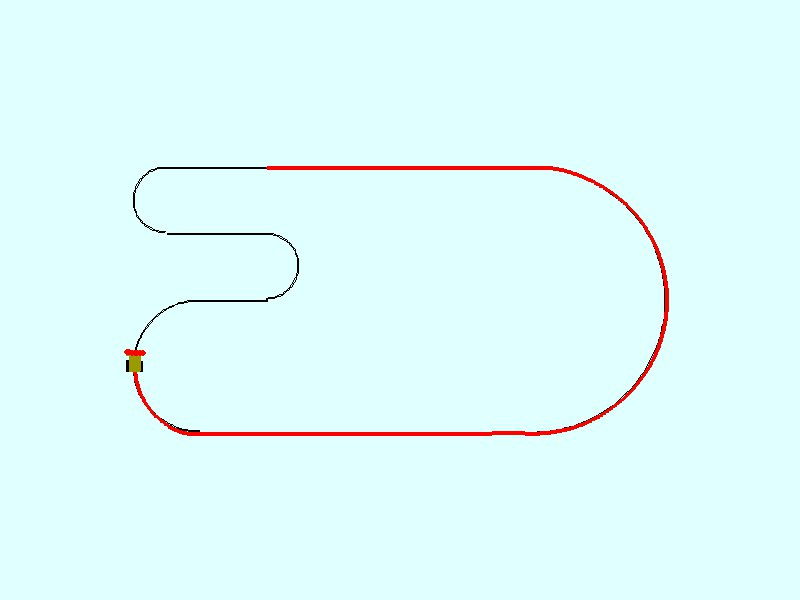
\includegraphics[width=2.8in]{./../code/results_q_learning/line_follower_solution.jpeg}
  \caption{\textit{Q-Learning} solution after more 700 iterations.}
  \label{img:qlearning_solution}
  \end{center}
\end{figure}

\section {Conclusion}

It was clear, therefore, that both implementation worked as expected. The \textit{Q-Learning} having a faster learning, converging to a local maximum with much less iteration than the \textit{SARSA} algorithm.

This makes \textit{Q-Learning} having a low variance but it might have a higher bias. While \textit{SARSA} have a higher viriance with a lower bias.

\vfill
\end{document}
